\documentclass[11pt,a4paper]{article}
\usepackage[utf8]{inputenc}
\usepackage[T1]{fontenc}
\usepackage[scaled=0.95]{helvet}
\renewcommand{\familydefault}{\sfdefault}
\usepackage{courier}
\usepackage[a4paper,top=2.5cm,bottom=2.5cm,left=2.5cm,right=2.5cm,headheight=14pt]{geometry}
\usepackage{amsmath}
\usepackage{xcolor}
\usepackage{graphicx}
\usepackage{tikz}
\usetikzlibrary{arrows.meta,positioning}
\usepackage{titlesec,fancyhdr,lastpage,booktabs,tabularx,enumitem,microtype,float,array,needspace}
\usepackage{caption}
\usepackage{subcaption}
\usepackage[colorlinks=true,linkcolor=azul,urlcolor=azul]{hyperref}

\definecolor{azul}{HTML}{1F4E99}
\definecolor{azulclaro}{HTML}{E9EFF8}

% Sin patrones de separación silábica en español en este entorno: se evita partir palabras
\hyphenpenalty=10000 \exhyphenpenalty=10000 \emergencystretch=3em \tolerance=2000
\renewcommand{\contentsname}{Índice}
\renewcommand{\tablename}{Tabla}
\renewcommand{\figurename}{Figura}
\captionsetup{font=small,labelfont={bf,color=azul},labelsep=period}
\captionsetup[sub]{font=small,labelfont=bf}

\titleformat{\section}{\needspace{7\baselineskip}\Large\bfseries}{\color{azul}\thesection}{0.7em}{}[{\color{azul}\titlerule[1pt]}]
\titleformat{\subsection}{\needspace{4\baselineskip}\large\bfseries\color{azul}}{\thesubsection}{0.6em}{}
\titlespacing*{\section}{0pt}{26pt}{10pt}
\titlespacing*{\subsection}{0pt}{12pt}{4pt}

\pagestyle{fancy}
\fancyhf{}
\fancyhead[L]{\small Reseñas de Amazon con MySQL, MongoDB y Neo4j}
\fancyhead[R]{\small\color{azul}Bases de Datos}
\fancyfoot[C]{\small \thepage\ / \pageref{LastPage}}
\renewcommand{\headrulewidth}{0.4pt}

\setlength{\parindent}{0pt}
\setlength{\parskip}{6pt}
\setlist{itemsep=2pt,topsep=4pt}
\newcommand{\code}[1]{\texttt{#1}}

\begin{document}

% ---------------- Portada ----------------
\begin{titlepage}

\vspace*{3.5cm}
{\large\color{azul}\bfseries Bases de Datos · Proyecto final}\\[14pt]
{\fontsize{30}{36}\selectfont\bfseries Reseñas de Amazon\\[2pt] con MySQL, MongoDB y Neo4j\par}
\vspace{12pt}
{\color{azul}\rule{0.55\linewidth}{2pt}}\\[12pt]
{\Large Diseño, carga, visualización y análisis en grafo\\ de unas 770.000 reseñas de productos\par}

\vfill
\begin{tabularx}{\linewidth}{@{}lX@{}}
\textbf{\color{azul}Autores} & Juan Tabuyo Castell\\
 & Jaime Tuesta de Simón\\[4pt]
\textbf{\color{azul}Titulación} & Grado en Ingeniería Matemática e Inteligencia Artificial (2.º curso)\\[4pt]
\textbf{\color{azul}Centro} & ICAI, Universidad Pontificia Comillas\\[4pt]
\textbf{\color{azul}Fecha} & Abril de 2026\\
\end{tabularx}
\vspace{1.5cm}
\end{titlepage}

\tableofcontents
\clearpage

% ---------------- Introducción ----------------
\section{Introducción}

El proyecto construye una plataforma de gestión y análisis de reseñas de Amazon que combina tres sistemas de bases de datos: MySQL para los datos estructurados, MongoDB para los textos y Neo4j para el análisis en forma de grafo. Se trabaja con los subconjuntos \emph{5-core} (cada usuario y cada producto tienen al menos cinco reseñas) de cuatro categorías: juguetes (167.597 reseñas), videojuegos (231.780), música digital (64.706) e instrumentos musicales (10.261). Más adelante se añade una quinta categoría, deportes y aire libre (296.337 reseñas).

Cada línea de los ficheros es un objeto JSON con una reseña: el identificador y el nombre del autor (\code{reviewerID}, \code{reviewerName}), el identificador del producto (\code{asin}), la nota (\code{overall}), los votos de utilidad (\code{helpful}), el texto y el resumen (\code{reviewText}, \code{summary}) y la fecha en dos formatos (\code{unixReviewTime}, \code{reviewTime}).

Todo el proyecto está escrito en Python, en seis módulos:

\begin{table}[H]
\centering
\small
\begin{tabularx}{\linewidth}{@{}>{\ttfamily}lX@{}}
\toprule
\normalfont\textbf{Módulo} & \textbf{Función}\\
\midrule
configuracion.py & Credenciales, nombres de las bases de datos y rutas de los ficheros.\\
load\_data.py & Creación de las bases de datos, tablas, colección e índices, y carga de los cuatro ficheros.\\
menu\_visualizacion.py & Menú de visualización sobre MySQL y MongoDB.\\
neo4JProyecto.py & Menú de análisis en grafo con Neo4j.\\
inserta\_dataset.py & Inserción de un nuevo dataset en la base de datos existente.\\
recomendacion\_populares.py & Recomendación de los artículos más populares no consumidos.\\
\bottomrule
\end{tabularx}
\end{table}

% ---------------- 1 ----------------
\section{Diseño y carga de datos}

\subsection{Esquema relacional (MySQL)}

La base de datos \code{ProyectoBBDD} de MySQL tiene tres tablas (claves primarias subrayadas):

\begin{itemize}
\item \textsc{usuarios}(\underline{reviewerID}, reviewerName)
\item \textsc{articulos}(\underline{asin}, categoria)
\item \textsc{reviews}(\underline{review\_id}, reviewerID, asin, overall, helpful\_1, helpful\_2, unixReviewTime, reviewTime, categoria)\\
con \code{reviewerID} clave foránea hacia \textsc{usuarios} y \code{asin} clave foránea hacia \textsc{articulos}.
\end{itemize}

\begin{figure}[H]
\centering
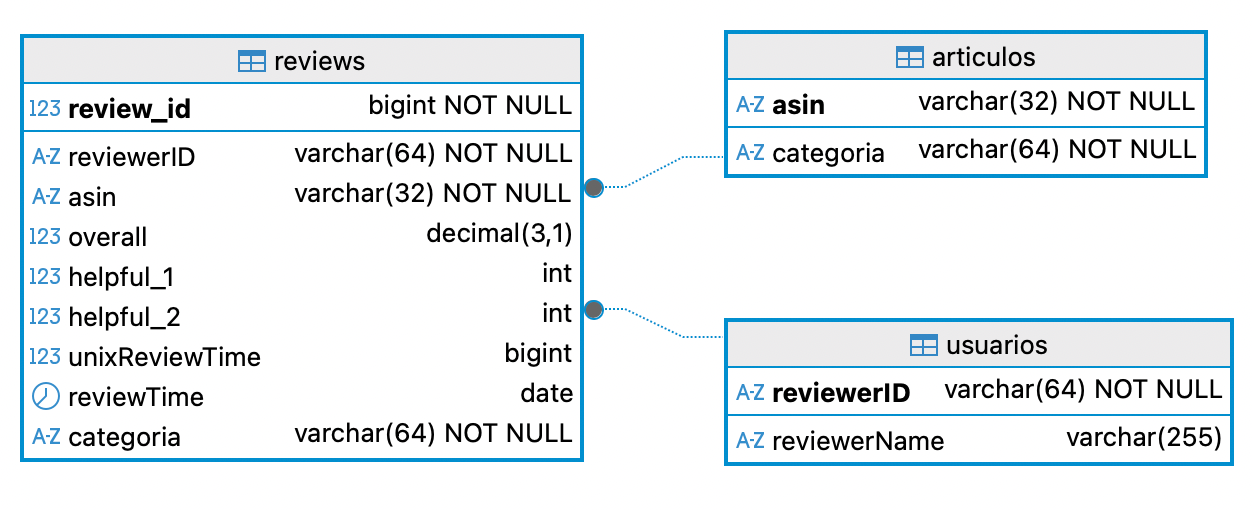
\includegraphics[width=0.85\linewidth]{figs/esquema_relacional.png}
\caption{Esquema relacional de la base de datos MySQL.}\label{fig:esquema}
\end{figure}

\subsection{Justificación del diseño}

\textbf{Separación en tres tablas.} Cada reseña del JSON original mezcla información de tres entidades distintas: el usuario que la escribe (\code{reviewerID}, \code{reviewerName}), el artículo reseñado (\code{asin}, categoría) y la propia reseña (nota, utilidad, fechas). Como un mismo usuario puede escribir reseñas en varias categorías y un mismo artículo puede recibir muchas reseñas, \textsc{usuarios} y \textsc{articulos} se extraen a tablas propias para evitar redundancia y cumplir la tercera forma normal. \textsc{reviews} queda como tabla de hechos con dos claves foráneas hacia ambas entidades.

\textbf{Clave primaria de \textsc{reviews}.} No hay garantía de que la pareja usuario--artículo, ni siquiera junto con la fecha, sea única en los datos. Por eso se añade un identificador autoincremental \code{review\_id} como clave primaria artificial, que además es más eficiente en los JOIN que una clave compuesta.

\textbf{Tipos de datos.} \code{reviewTime} se convierte del texto «MM DD, YYYY» al tipo \code{DATE}, como exige el enunciado. \code{unixReviewTime} se mantiene como \code{BIGINT} porque permite ordenar cronológicamente sin conversiones. La nota se guarda como \code{DECIMAL(3,1)} y el campo \code{helpful} se desdobla en dos enteros (\code{helpful\_1}, votos útiles, y \code{helpful\_2}, votos totales) para poder consultarlos por separado.

\textbf{Categoría en \textsc{reviews}.} La categoría está en \textsc{articulos}, pero se repite en \textsc{reviews} para filtrar por categoría en las visualizaciones sin necesidad de un JOIN. Es una desnormalización controlada, justificada por el patrón de consultas esperado.

\subsection{Reparto entre MySQL y MongoDB}

En \textbf{MySQL} se almacena toda la información estructurada y numérica: identificadores (\code{reviewerID}, \code{asin}, \code{review\_id}), nombre del usuario, categoría, nota, utilidad y las dos fechas. Son datos de tamaño fijo, con relaciones claras entre entidades, sobre los que se hacen consultas relacionales (JOIN, GROUP BY, agregaciones por año, categoría o usuario) para las gráficas del menú de visualización.

En \textbf{MongoDB} (colección \code{reviews\_texto}) se almacenan los campos de texto libre, \code{reviewText} y \code{summary}, junto con \code{reviewerID}, \code{asin}, \code{unixReviewTime} y la categoría como metadatos para poder filtrar y relacionar cada documento con su reseña. Son campos de longitud muy variable y contenido no estructurado, que encajan mejor en una base de datos documental. En el proyecto se usan para la nube de palabras por categoría, que se resuelve con una consulta \code{find} que proyecta \code{summary}, sin necesidad de JOIN.

De este modo, todos los campos del JSON original quedan almacenados: MySQL concentra los datos sobre los que se hacen consultas relacionales, y MongoDB, los campos textuales.

\subsection{Carga de datos e índices}

La creación de la base de datos, las tablas, la colección y los índices, y la inserción de los datos, se realizan desde Python ejecutando \code{load\_data.py}. Las credenciales, los nombres de las bases de datos y las rutas de los ficheros se definen en \code{configuracion.py}, de modo que basta con modificar ese fichero para cargar los datos en otro equipo.

Los ficheros se leen \textbf{línea a línea} con un generador, sin cargar nunca el fichero completo en memoria, y las inserciones se agrupan en lotes de 5.000 reseñas (\code{executemany} en MySQL e \code{insert\_many} en MongoDB) para reducir el número de viajes a cada base de datos. Como un mismo usuario puede tener reseñas en varias categorías, antes de cargar cada fichero se leen los usuarios y artículos ya existentes y se mantienen en conjuntos, de forma que cada usuario y cada artículo se insertan una sola vez.

Al terminar la carga se crean índices para acelerar las consultas de visualización:

\begin{itemize}
\item MySQL (tabla \textsc{reviews}): \code{categoria}, \code{asin}, \code{reviewerID}, \code{overall} y \code{unixReviewTime}.
\item MongoDB (colección \code{reviews\_texto}): \code{categoria}, \code{reviewerID} y \code{asin}.
\end{itemize}

% ---------------- 2 ----------------
\section{Aplicación de acceso y visualización}

La aplicación \code{menu\_visualizacion.py} permite consultar y visualizar distintos aspectos de los datos mediante un menú por terminal que se repite hasta que el usuario elige salir (Figura~\ref{fig:menuvis}). Las categorías disponibles se leen de la propia base de datos al arrancar, de modo que la aplicación incluye automáticamente las que se añadan después.

\begin{figure}[H]
\centering
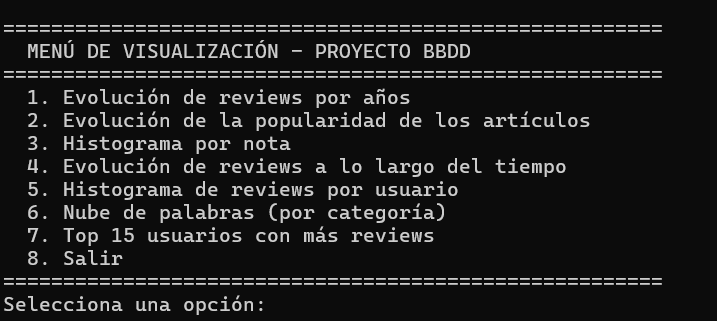
\includegraphics[width=0.6\linewidth]{figs/menu_visualizacion.png}
\caption{Menú de visualización.}\label{fig:menuvis}
\end{figure}

El menú ofrece siete gráficas:

\begin{enumerate}
\item \textbf{Reseñas por año}, por categoría o para todas.
\item \textbf{Evolución de la popularidad}: artículos ordenados de mayor a menor número de reseñas.
\item \textbf{Histograma por nota}, por categoría, para todas o para un artículo concreto. Si el artículo introducido no existe, se informa al usuario.
\item \textbf{Evolución de las reseñas a lo largo del tiempo}: número acumulado de reseñas de cada categoría.
\item \textbf{Histograma de reseñas por usuario}: cuántos usuarios han escrito cada número de reseñas.
\item \textbf{Nube de palabras por categoría}, a partir del campo \code{summary} de MongoDB, considerando solo las palabras de más de tres letras y generada con la librería \code{wordcloud}.
\item \textbf{Los 15 usuarios con más reseñas}, como visualización adicional.
\end{enumerate}

Las consultas numéricas se realizan sobre MySQL, que almacena los campos necesarios para filtros, agrupaciones y ordenaciones, y la nube de palabras, sobre MongoDB. Las Figuras~\ref{fig:vis1}--\ref{fig:vis3} muestran las gráficas obtenidas con todos los productos.

\begin{figure}[H]
\centering
\begin{subfigure}[t]{0.49\linewidth}\centering
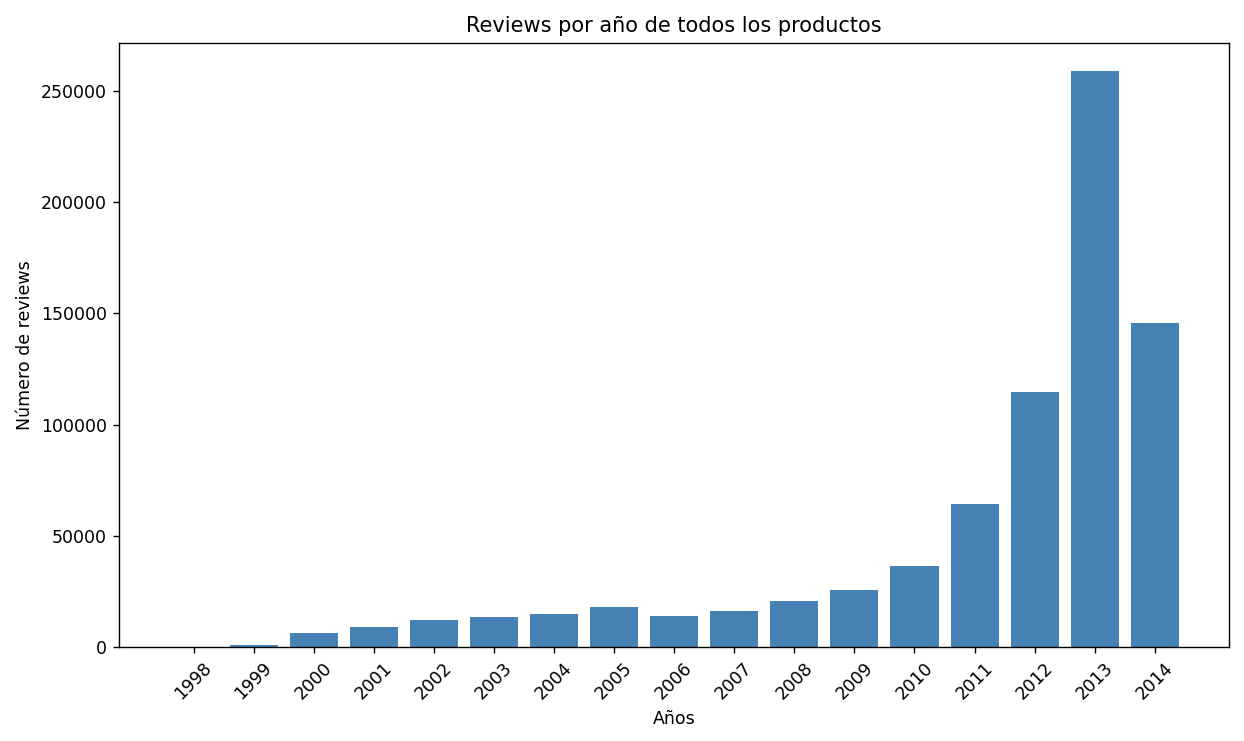
\includegraphics[width=\linewidth]{figs/reviews_por_anio.png}
\caption{Reseñas por año.}
\end{subfigure}\hfill
\begin{subfigure}[t]{0.49\linewidth}\centering
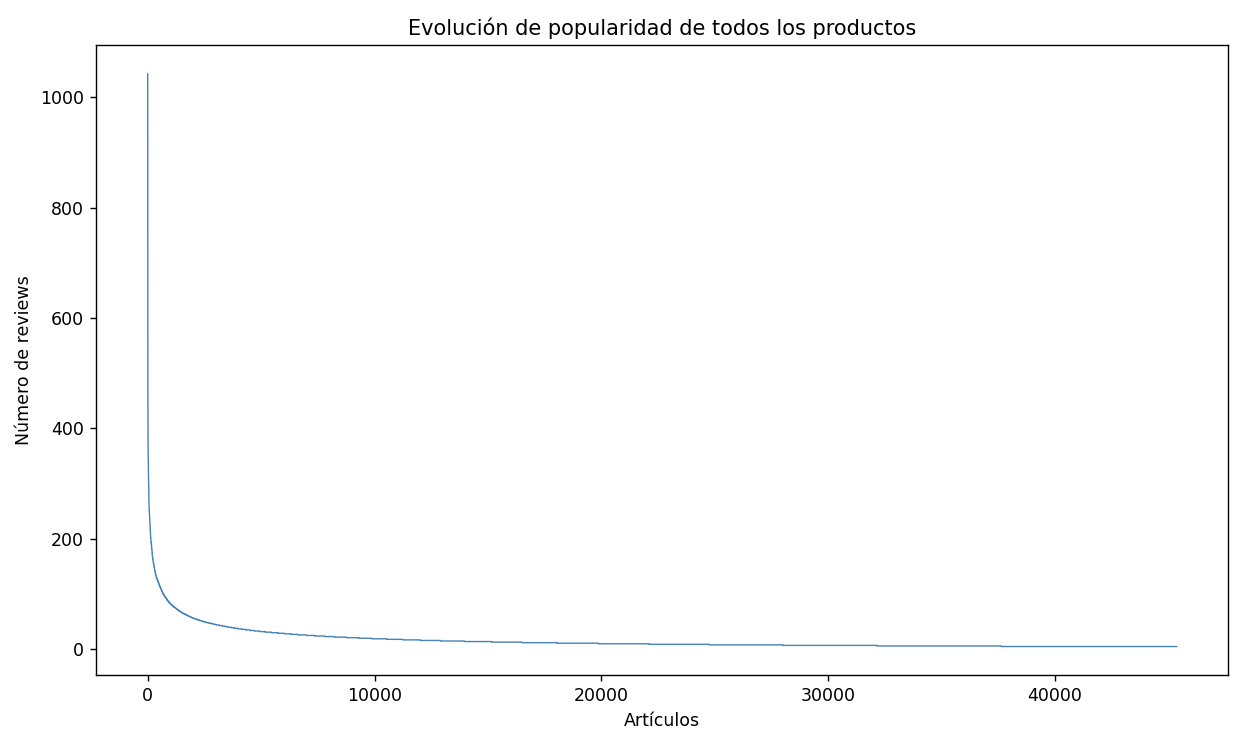
\includegraphics[width=\linewidth]{figs/popularidad_articulos.png}
\caption{Popularidad de los artículos.}
\end{subfigure}
\caption{Reseñas por año y evolución de la popularidad de los artículos.}\label{fig:vis1}
\end{figure}

\begin{figure}[H]
\centering
\begin{subfigure}[t]{0.42\linewidth}\centering
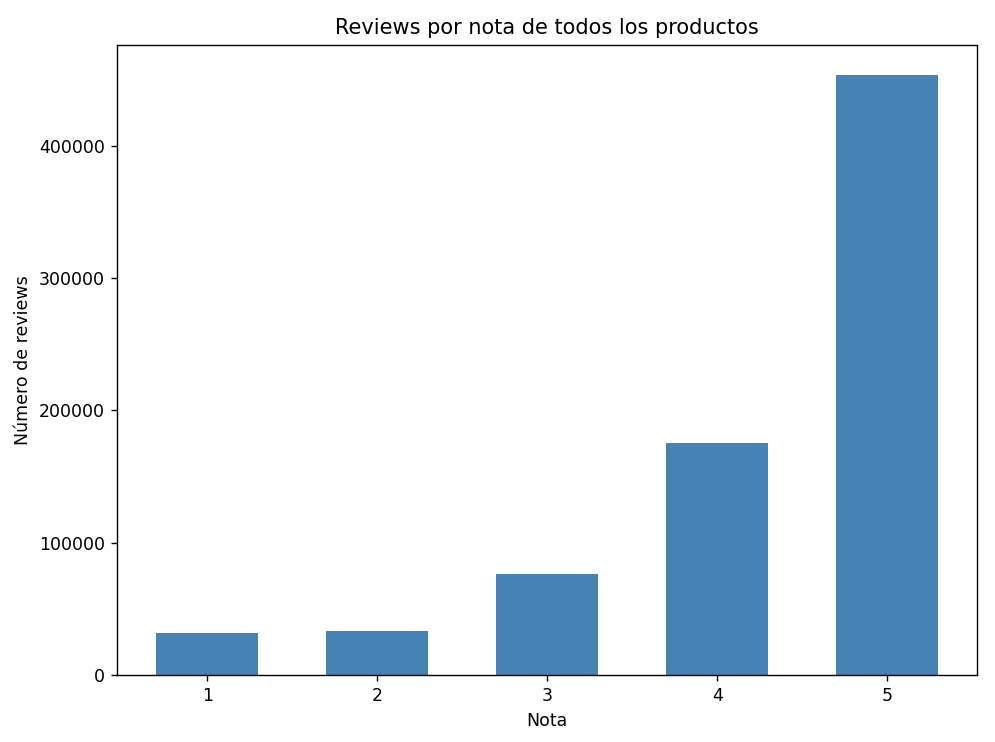
\includegraphics[width=\linewidth]{figs/reviews_por_nota.png}
\caption{Reseñas por nota.}
\end{subfigure}\hfill
\begin{subfigure}[t]{0.56\linewidth}\centering
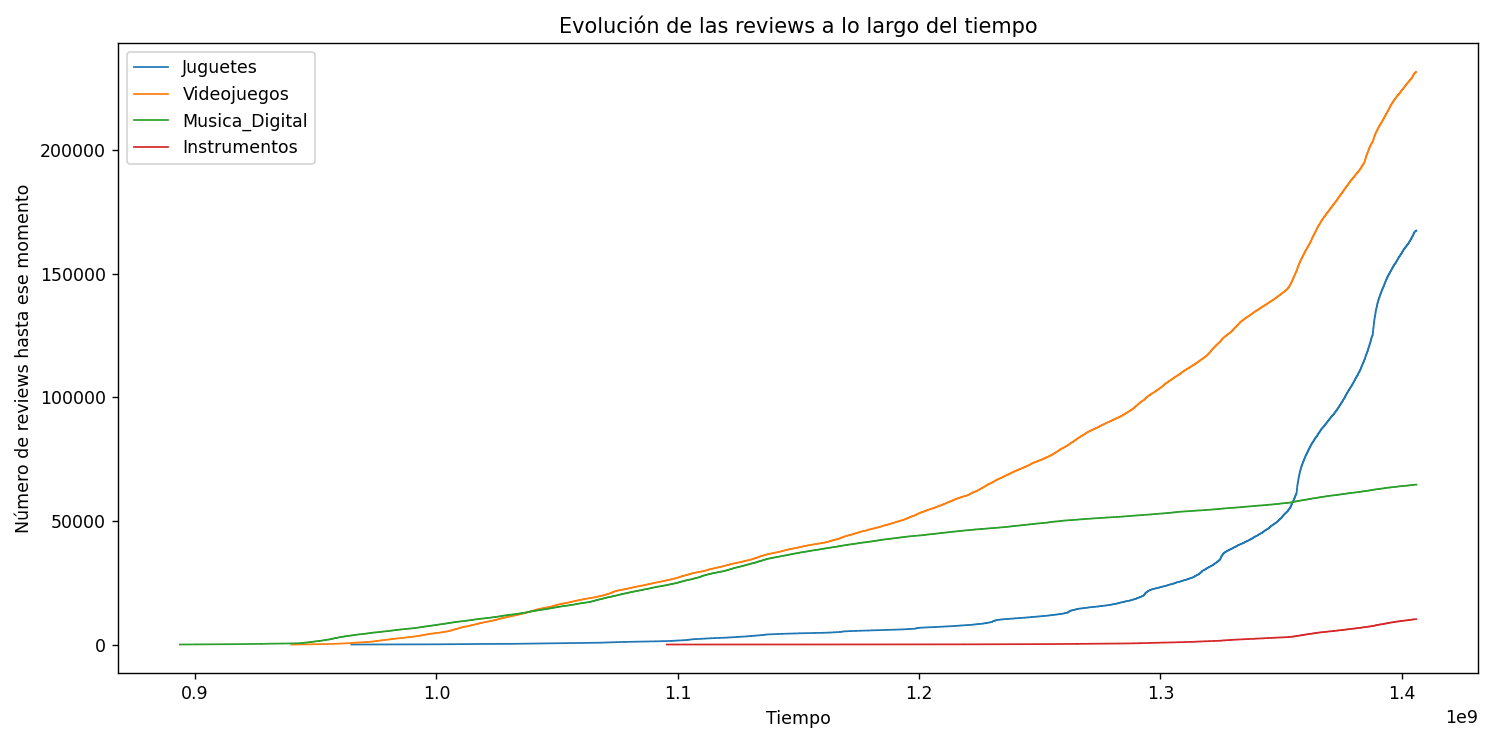
\includegraphics[width=\linewidth]{figs/evolucion_temporal.png}
\caption{Evolución de las reseñas a lo largo del tiempo.}
\end{subfigure}
\caption{Histograma por nota y evolución acumulada de las reseñas por categoría.}\label{fig:vis2}
\end{figure}

\begin{figure}[H]
\centering
\begin{subfigure}[t]{0.49\linewidth}\centering
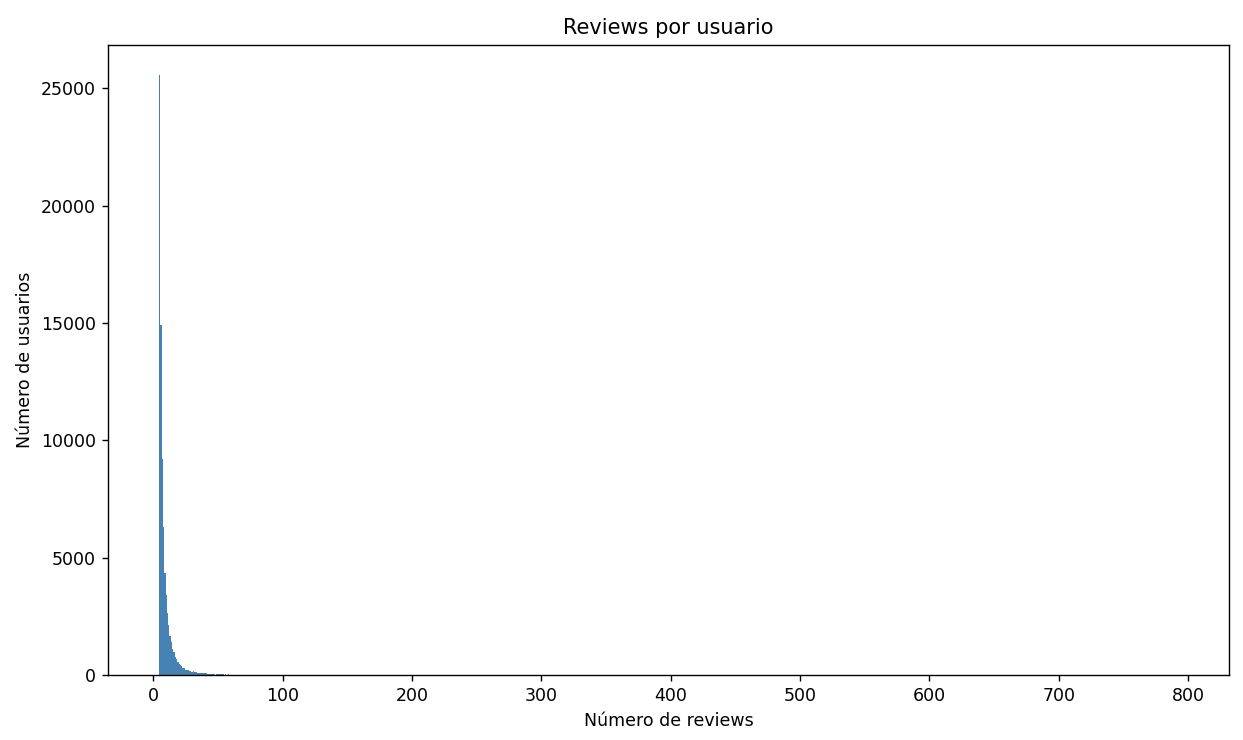
\includegraphics[width=\linewidth]{figs/reviews_por_usuario.png}
\caption{Reseñas por usuario.}
\end{subfigure}\hfill
\begin{subfigure}[t]{0.49\linewidth}\centering
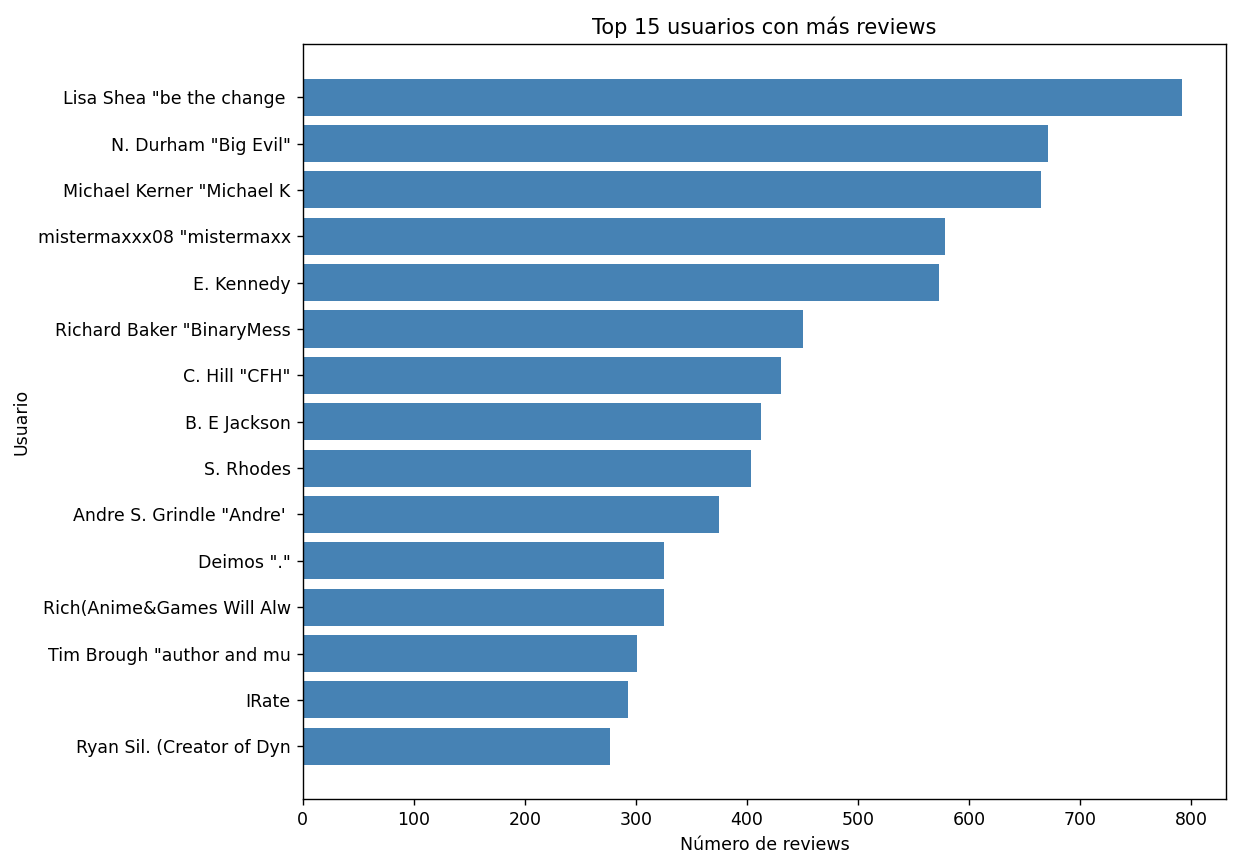
\includegraphics[width=\linewidth]{figs/top15_usuarios.png}
\caption{Los 15 usuarios con más reseñas.}
\end{subfigure}

\vspace{8pt}
\begin{subfigure}[t]{0.62\linewidth}\centering
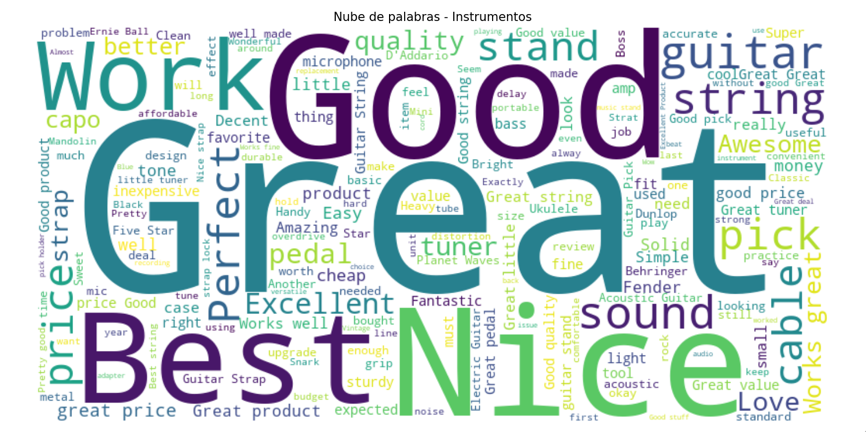
\includegraphics[width=\linewidth]{figs/nube_palabras_instrumentos.png}
\caption{Nube de palabras de la categoría de instrumentos.}
\end{subfigure}
\caption{Reseñas por usuario, usuarios más activos y nube de palabras.}\label{fig:vis3}
\end{figure}

% ---------------- 3 ----------------
\section{Análisis en grafo con Neo4j}

La aplicación \code{neo4JProyecto.py} es otro menú por terminal (Figura~\ref{fig:menuneo}) que obtiene datos de MySQL y los carga en Neo4j con distintas representaciones en forma de grafo. Cada opción limpia antes la base de datos de Neo4j para no mezclar resultados y, al terminar la carga, avisa al usuario para que pueda consultarla en Neo4j Browser.

\begin{figure}[H]
\centering
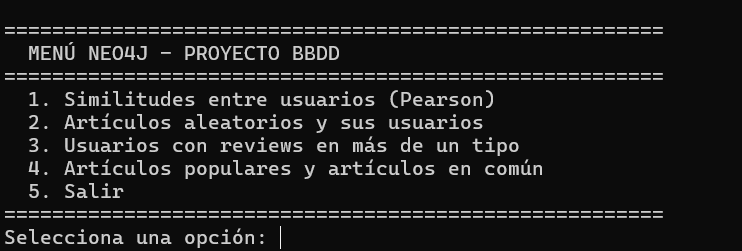
\includegraphics[width=0.6\linewidth]{figs/menu_neo4j.png}
\caption{Menú de Neo4j.}\label{fig:menuneo}
\end{figure}

\subsection{Similitud entre usuarios}

Se obtienen los 30 usuarios con más reseñas (el número se define en \code{configuracion.py}) y se calcula la similitud entre cada par mediante la correlación de Pearson sobre los artículos que ambos han puntuado:
\[
PC(u,v)=\frac{\sum_{i\in I_{uv}}(r_{ui}-\bar r_u)(r_{vi}-\bar r_v)}{\sqrt{\sum_{i\in I_{uv}}(r_{ui}-\bar r_u)^2}\,\sqrt{\sum_{i\in I_{uv}}(r_{vi}-\bar r_v)^2}},
\]
donde $I_{uv}$ es el conjunto de artículos puntuados por ambos usuarios y $\bar r_u$, $\bar r_v$ son las medias de todas las valoraciones de cada usuario. Solo se guardan las similitudes de los pares con algún artículo en común. En Neo4j, cada usuario es un nodo y cada similitud, una relación con su valor; como la similitud es simétrica, se crea una relación por par y se consulta sin dirección. Una consulta Cypher muestra por pantalla el usuario con más vecinos.

\subsection{Artículos aleatorios y sus usuarios}

El usuario elige una categoría y un número $n$ de artículos, que se seleccionan al azar. Se cargan en Neo4j esos artículos y todos los usuarios que los han puntuado, unidos por relaciones \code{HA\_PUNTUADO} con la nota y el momento de la reseña como propiedades.

\subsection{Usuarios de varias categorías}

Se toman los 400 primeros usuarios ordenados por nombre y se seleccionan los que han puntuado artículos de al menos dos categorías distintas. En Neo4j se representan como nodos de usuario enlazados con nodos de tipo de artículo, y cada enlace indica cuántos artículos de ese tipo ha puntuado el usuario.

\subsection{Artículos populares y artículos en común}

Se seleccionan los 5 artículos más populares de entre los que tienen menos de 40 reseñas y se cargan con todos los usuarios que los han puntuado. Además, se crean enlaces entre cada par de usuarios con artículos en común, con el número de artículos compartidos como propiedad.

\begin{figure}[H]
\centering
\begin{subfigure}[t]{0.49\linewidth}\centering
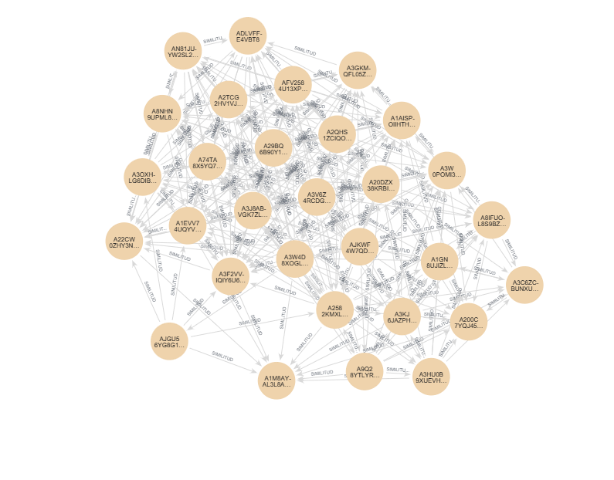
\includegraphics[width=0.92\linewidth]{figs/neo4j_similitudes.png}
\caption{Similitud entre los 30 usuarios con más reseñas.}
\end{subfigure}\hfill
\begin{subfigure}[t]{0.49\linewidth}\centering
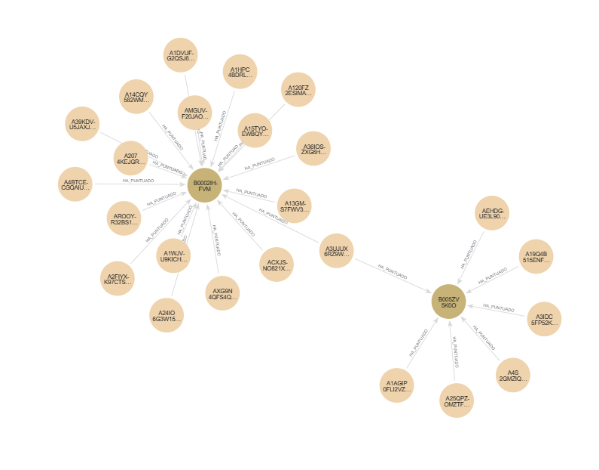
\includegraphics[width=0.92\linewidth]{figs/neo4j_articulos_aleatorios.png}
\caption{Artículos aleatorios y sus usuarios.}
\end{subfigure}

\vspace{8pt}
\begin{subfigure}[t]{0.49\linewidth}\centering
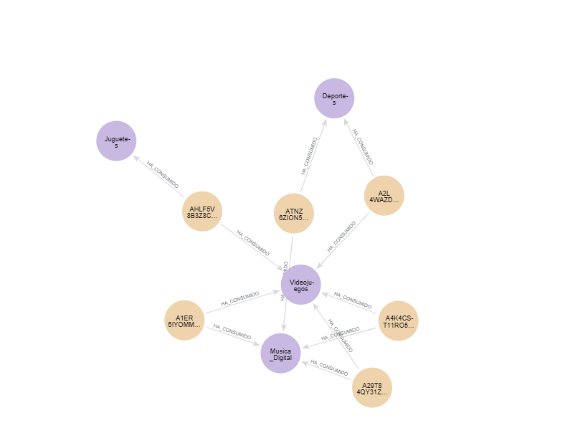
\includegraphics[width=0.92\linewidth]{figs/neo4j_multicategoria.png}
\caption{Usuarios con reseñas en varias categorías.}
\end{subfigure}\hfill
\begin{subfigure}[t]{0.49\linewidth}\centering
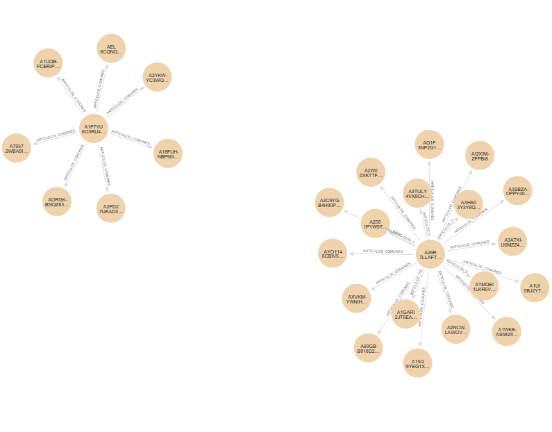
\includegraphics[width=0.92\linewidth]{figs/neo4j_populares.png}
\caption{Artículos populares y usuarios con artículos en común.}
\end{subfigure}
\caption{Grafos obtenidos en Neo4j Browser con cada opción del menú.}\label{fig:neo}
\end{figure}

% ---------------- 4 ----------------
\section{Inserción de nuevos datos}

El script \code{inserta\_dataset.py} añade un nuevo dataset a la base de datos ya creada, sin eliminar ni modificar los datos existentes. Se ha elegido el fichero de deportes y aire libre (\emph{Sports and Outdoors}), que se incorpora como categoría «Deportes».

El proceso comienza con dos validaciones: que el fichero exista en la ruta configurada y que la categoría no esté ya en la base de datos, para evitar cargar dos veces el mismo dataset. A continuación se leen los identificadores de los usuarios y artículos existentes. Como un mismo usuario puede haber escrito reseñas en distintas categorías, los usuarios y artículos que ya estaban se reutilizan y solo se insertan los nuevos; todas las reseñas del fichero se insertan en MySQL y MongoDB con la misma estructura que en la carga inicial. Al terminar, el programa muestra cuántas reseñas, usuarios nuevos, usuarios reutilizados y artículos nuevos se han insertado, y el estado global de la base de datos.

% ---------------- 5 ----------------
\section{Visualización con Power BI y recomendación}

\subsection{Gráficas en Power BI}

Tres de las gráficas obtenidas con Python (reseñas por año, histograma por nota y los 15 usuarios con más reseñas) se han reproducido con Power BI (Figura~\ref{fig:pbi}).

\begin{figure}[H]
\centering
\begin{subfigure}[t]{0.49\linewidth}\centering
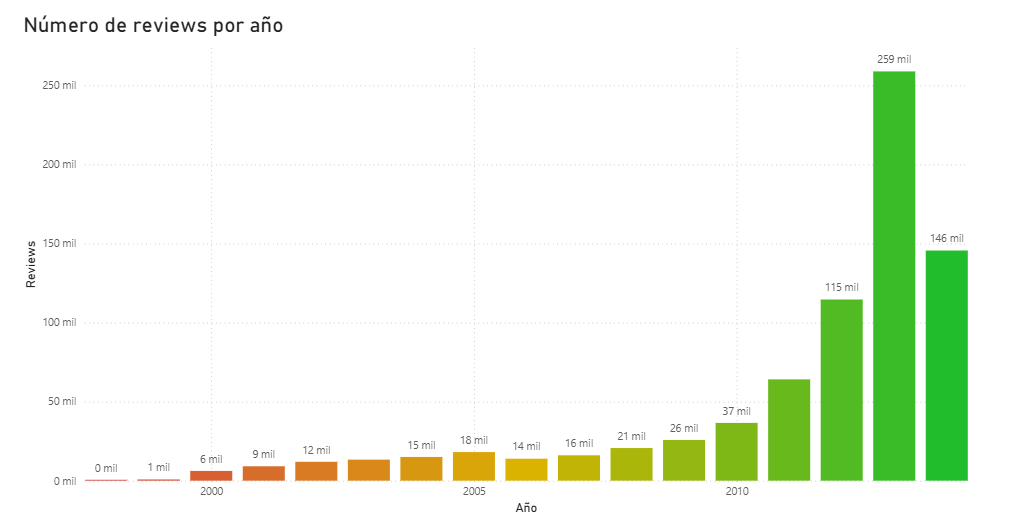
\includegraphics[width=\linewidth]{figs/powerbi_reviews_por_anio.png}
\caption{Reseñas por año.}
\end{subfigure}\hfill
\begin{subfigure}[t]{0.49\linewidth}\centering
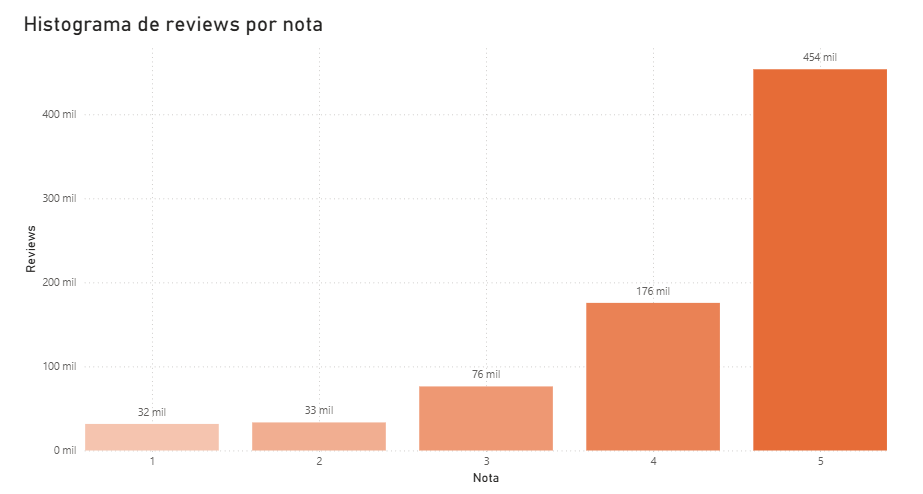
\includegraphics[width=\linewidth]{figs/powerbi_reviews_por_nota.png}
\caption{Reseñas por nota.}
\end{subfigure}

\vspace{8pt}
\begin{subfigure}[t]{0.62\linewidth}\centering
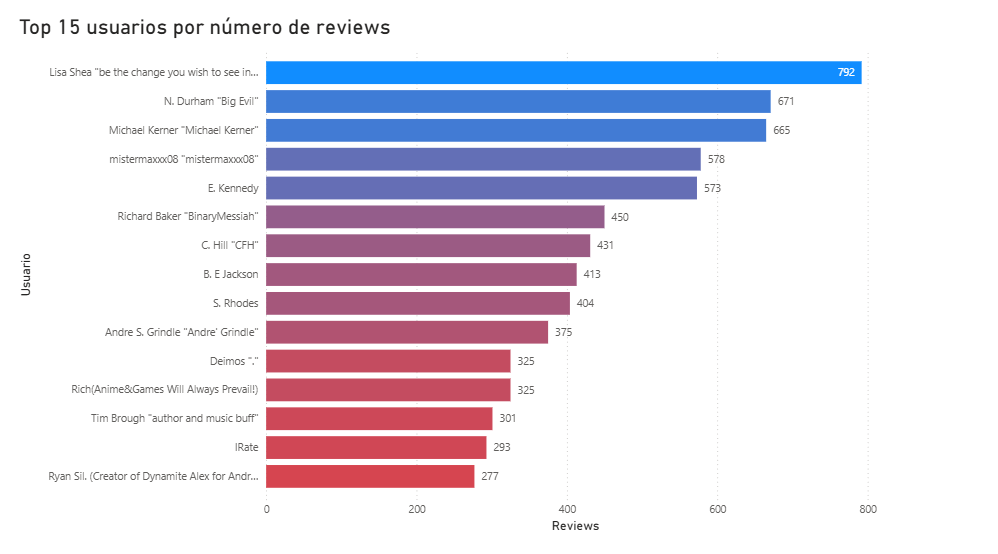
\includegraphics[width=\linewidth]{figs/powerbi_top15_usuarios.png}
\caption{Los 15 usuarios con más reseñas.}
\end{subfigure}
\caption{Gráficas reproducidas con Power BI.}\label{fig:pbi}
\end{figure}

\subsection{Modelo de recomendación propuesto}

Se propone un sistema de recomendación que sugiera a cada usuario artículos que todavía no ha consumido, utilizando principalmente los datos estructurados de MySQL (\code{reviewerID}, \code{asin}, \code{overall}, \code{categoria}). A partir de estas interacciones se construiría una matriz usuario--artículo, cuyos valores serían las notas (vacíos si no hay interacción), y se aplicaría un modelo de filtrado colaborativo, que permite predecir qué productos pueden interesar a un usuario a partir de sus valoraciones previas y de patrones de comportamiento similares.

Con las predicciones, se eliminarían los artículos ya consumidos por el usuario y se generaría un ranking con las recomendaciones más relevantes, con la opción de filtrar por categoría. Como mecanismo de respaldo para usuarios con poco historial, se recurriría a la popularidad por categoría, devolviendo los artículos más populares que el usuario aún no haya consumido. La Figura~\ref{fig:ml} resume el proceso.

\begin{figure}[H]
\centering
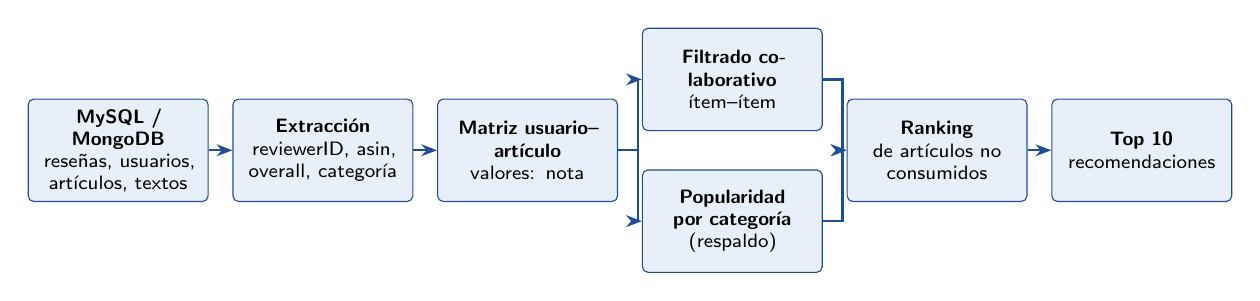
\begin{tikzpicture}[
  caja/.style={draw=azul,fill=azulclaro,rounded corners=2pt,align=center,font=\scriptsize,minimum height=1.3cm,text width=2.05cm},
  flecha/.style={-{Stealth[length=2mm]},thick,azul}]
\node[caja] (db) at (0,0) {\textbf{MySQL / MongoDB}\\ reseñas, usuarios, artículos, textos};
\node[caja] (ext) at (2.6,0) {\textbf{Extracción}\\ reviewerID, asin, overall, categoría};
\node[caja] (mat) at (5.2,0) {\textbf{Matriz usuario--artículo}\\ valores: nota};
\node[caja] (cf) at (7.8,0.9) {\textbf{Filtrado colaborativo}\\ ítem--ítem};
\node[caja] (pop) at (7.8,-0.9) {\textbf{Popularidad por categoría}\\ (respaldo)};
\node[caja] (rank) at (10.4,0) {\textbf{Ranking}\\ de artículos no consumidos};
\node[caja] (top) at (13.0,0) {\textbf{Top 10}\\ recomendaciones};
\draw[flecha] (db) -- (ext);
\draw[flecha] (ext) -- (mat);
\draw[flecha] (mat.east) -- ++(0.25,0) |- (cf.west);
\draw[flecha] (mat.east) -- ++(0.25,0) |- (pop.west);
\draw[flecha] (cf.east) -- ++(0.25,0) |- (rank.west);
\draw[flecha] (pop.east) -- ++(0.25,0) |- (rank.west);
\draw[flecha] (rank) -- (top);
\end{tikzpicture}
\caption{Diagrama del modelo de recomendación propuesto.}\label{fig:ml}
\end{figure}

\subsection{Recomendación de artículos populares no consumidos}

El script \code{recomendacion\_populares.py} implementa el mecanismo de respaldo: dado el identificador original de un usuario y una categoría, devuelve los 10 artículos más populares de esa categoría que el usuario todavía no ha consumido. Se resuelve con una única consulta SQL sobre \textsc{reviews} que filtra por categoría, excluye con \code{NOT EXISTS} los artículos que el usuario ya ha reseñado, agrupa por artículo y ordena por número de reseñas (con la nota media y el \code{asin} como criterios de desempate, para que el resultado sea estable). El programa comprueba antes que el usuario exista y ofrece las categorías disponibles en la base de datos.

\begin{figure}[H]
\centering
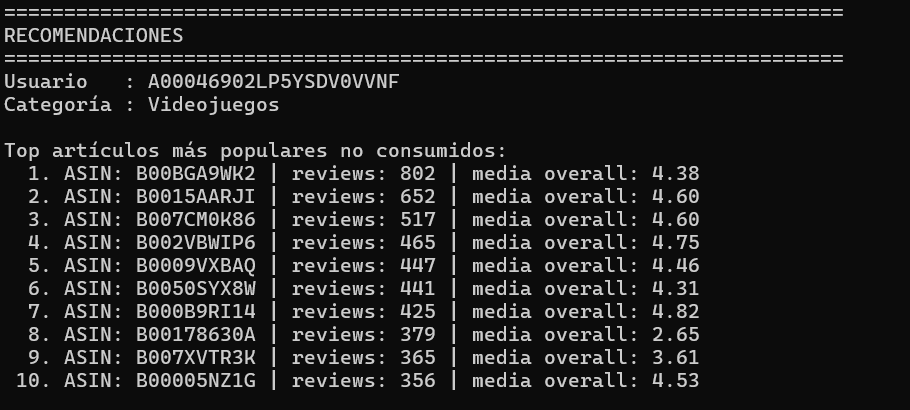
\includegraphics[width=0.72\linewidth]{figs/recomendaciones_top10.png}
\caption{Diez recomendaciones de la categoría de videojuegos para un usuario.}\label{fig:recom}
\end{figure}

\end{document}
